\documentclass[10pt,utf8]{beamer}

\mode<presentation> {
%  \usetheme{Boadilla}
  \usetheme{Madrid}
%	\usetheme{Fzu}
  \setbeamercovered{transparent}
}

\usepackage{palatino}
\usepackage{graphicx}
\usepackage{array}
\usepackage{color}
\usepackage{subfigure}
\usepackage{colortbl}
\usepackage{amsmath}
\usepackage{hyperref}
%\usepackage{tikz}
%\usetikzlibrary{arrows,shapes,backgrounds}


%\definecolor{MyDarkGreen}{rgb}{0.3,0.7,0.3}

\title{Feeding ML models with the data from the databases in real-time}
\author{Vojtěch Juránek}
\institute[Red Hat]{Red Hat}
\date{Feb. 3rd 2024, FOSDEM, Brussels}

\newenvironment{mylisting}
{\begin{list}{}{\setlength{\leftmargin}{1em}}\item\scriptsize\bfseries}
{\end{list}}

\newenvironment{mytinylisting}
{\begin{list}{}{\setlength{\leftmargin}{1em}}\item\tiny\bfseries}
{\end{list}}


\begin{document}

%\tikzstyle{every picture}+=[remember picture]
%\tikzstyle{na} = [baseline=-.5ex]


\begin{frame}
 \titlepage
\end{frame}


\begin{frame}
    \begin{figure}
        \centering
        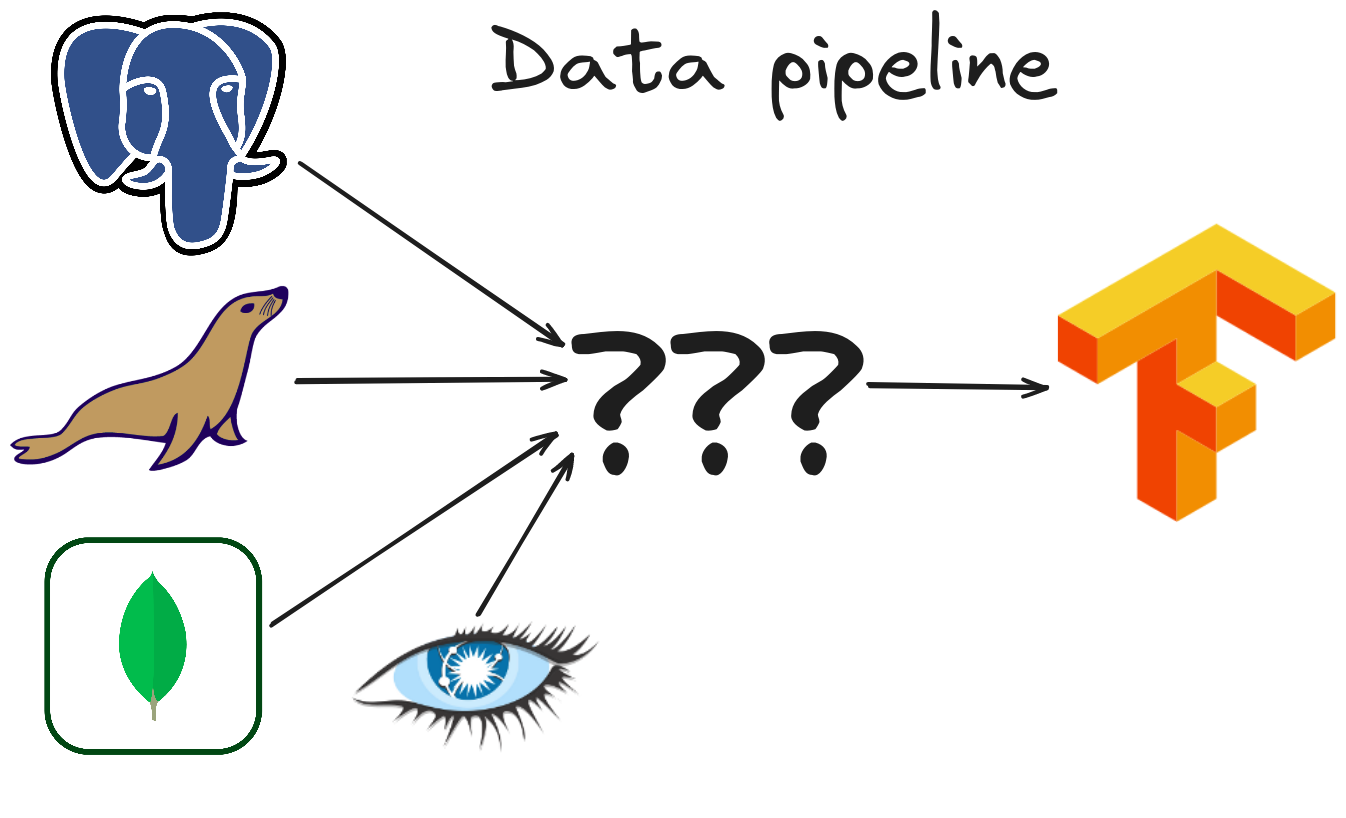
\includegraphics[height=8cm]{./img/dbs_to_tf.eps}
    \end{figure}
\end{frame}

\begin{frame}
    \frametitle{Change Data Capture (CDC)}
%     \begin{figure}
%         \centering
%         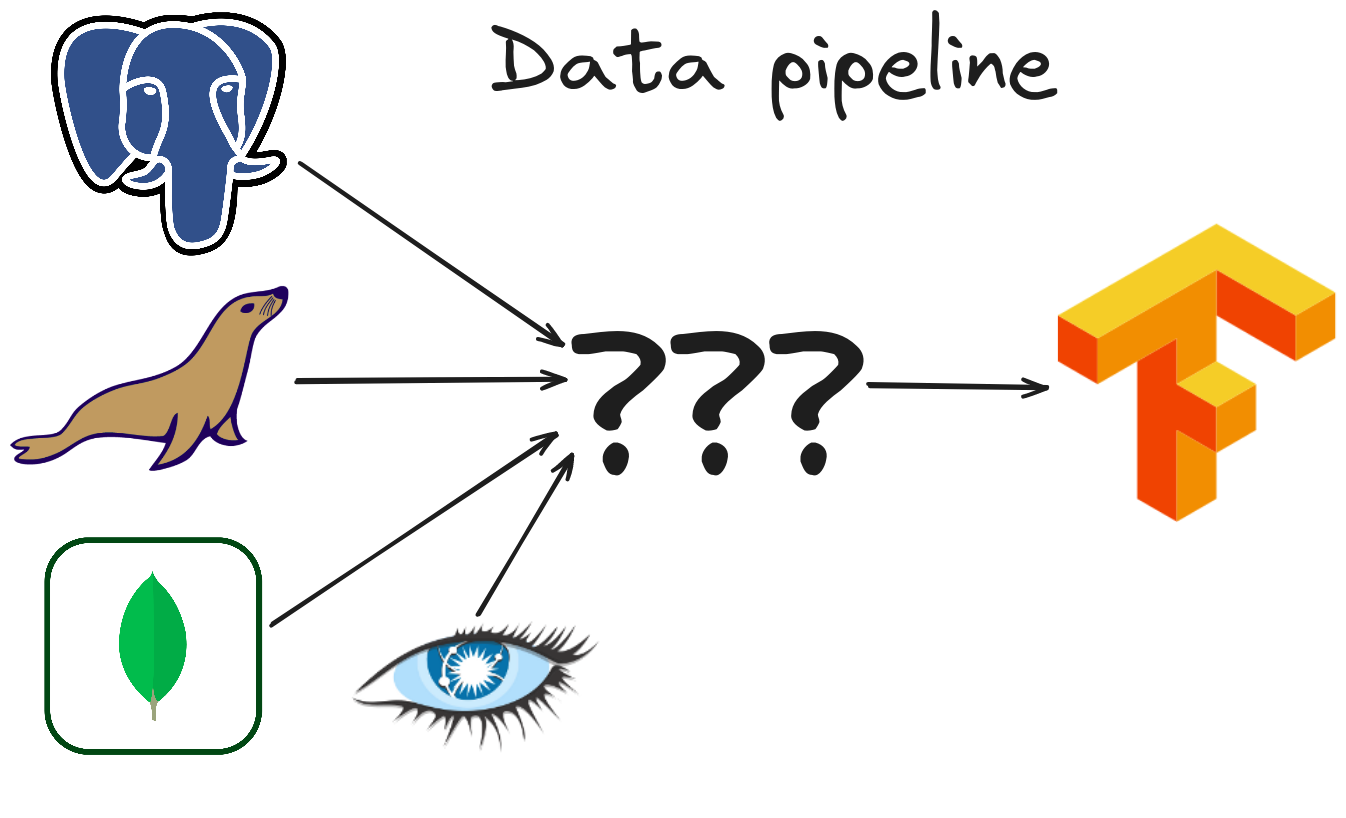
\includegraphics[height=8cm]{./img/dbs_to_tf.eps}
%     \end{figure}
\end{frame}

\begin{frame}
    \frametitle{Debezium}
%     \begin{figure}
%         \centering
%         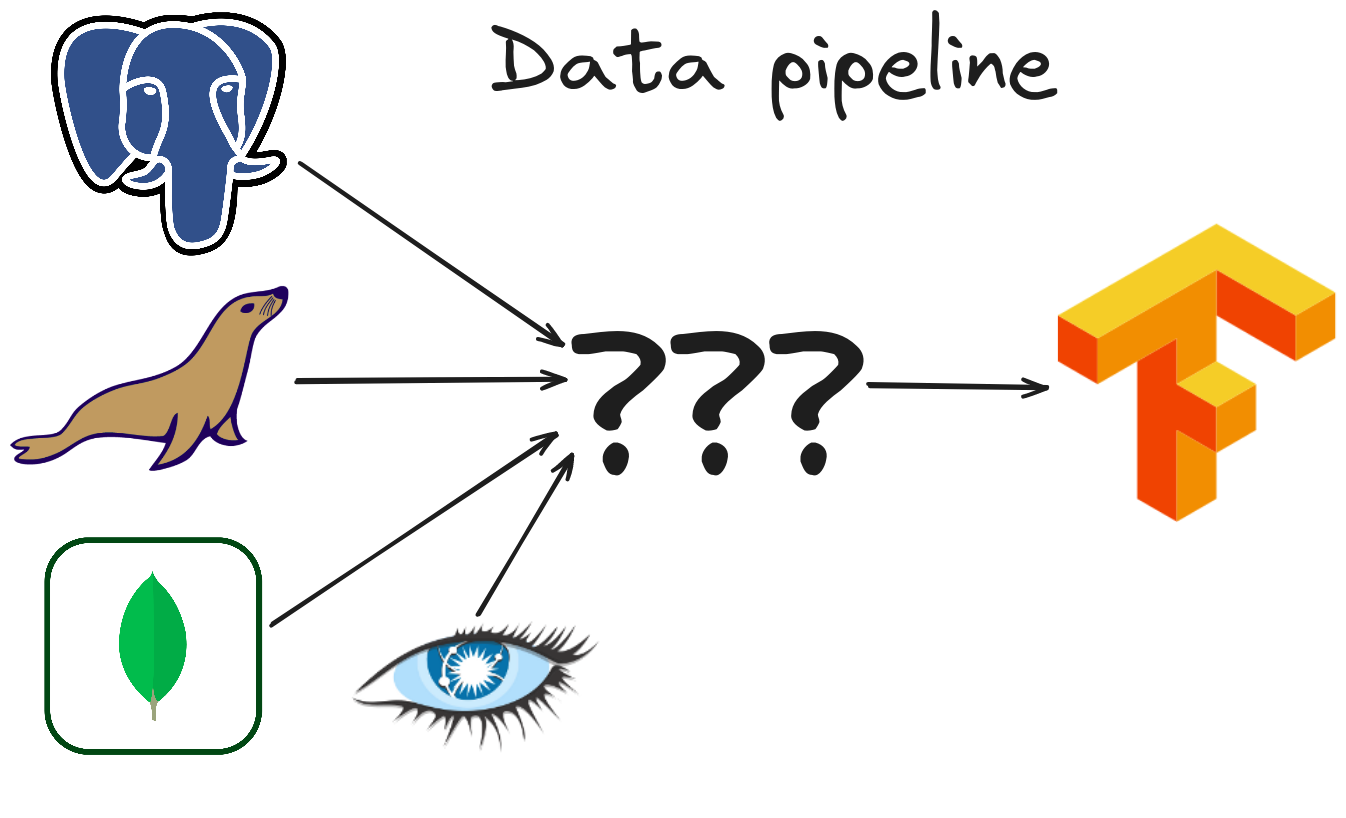
\includegraphics[height=8cm]{./img/dbs_to_tf.eps}
%     \end{figure}
\end{frame}

\end{document}
